\documentclass[reprint,english,notitlepage, nofootinbib]{revtex4-1}  % defines the basic parameters of the document

% if you want a single-column, remove reprint

% allows special characters (including æøå)
\usepackage[utf8]{inputenc}
\usepackage[english]{babel}

%% note that you may need to download some of these packages manually, it depends on your setup.
%% I recommend downloading TeXMaker, because it includes a large library of the most common packages.

\usepackage{physics,amssymb}  % mathematical symbols (physics imports amsmath)
\usepackage{graphicx}         % include graphics such as plots
\usepackage{xcolor}           % set colors
\usepackage{hyperref}         % automagic cross-referencing (this is GODLIKE)
\usepackage{tikz}             % draw figures manually
\usepackage{standalone}
\usepackage{listings}         % display code
\usepackage{subfigure} 
\usepackage{float}       % imports a lot of cool and useful figure commands

% defines the color of hyperref objects
% Blending two colors:  blue!80!black  =  80% blue and 20% black
\hypersetup{ % this is just my personal choice, feel free to change things
    colorlinks,
    linkcolor={red!50!black},
    citecolor={blue!50!black},
    urlcolor={blue!80!black}}

%% Defines the style of the programming listing
%% This is actually my personal template, go ahead and change stuff if you want
\lstset{ %
	inputpath=,
	backgroundcolor=\color{white!88!black},
	basicstyle={\ttfamily\scriptsize},
	commentstyle=\color{magenta},
	language=Python,
	morekeywords={True,False},
	tabsize=4,
	stringstyle=\color{green!55!black},
	frame=single,
	keywordstyle=\color{blue},
	showstringspaces=false,
	columns=fullflexible,
	keepspaces=true}


%% USEFUL LINKS:
%%
%%   UiO LaTeX guides:        https://www.mn.uio.no/ifi/tjenester/it/hjelp/latex/ 
%%   mathematics:             https://en.wikibooks.org/wiki/LaTeX/Mathematics

%%   PHYSICS !                https://mirror.hmc.edu/ctan/macros/latex/contrib/physics/physics.pdf

%%   the basics of Tikz:       https://en.wikibooks.org/wiki/LaTeX/PGF/TikZ
%%   all the colors!:          https://en.wikibooks.org/wiki/LaTeX/Colors
%%   how to draw tables:       https://en.wikibooks.org/wiki/LaTeX/Tables
%%   code listing styles:      https://en.wikibooks.org/wiki/LaTeX/Source_Code_Listings
%%   \includegraphics          https://en.wikibooks.org/wiki/LaTeX/Importing_Graphics
%%   learn more about figures  https://en.wikibooks.org/wiki/LaTeX/Floats,_Figures_and_Captions
%%   automagic bibliography:   https://en.wikibooks.org/wiki/LaTeX/Bibliography_Management  (this one is kinda difficult the first time)
%%   REVTeX Guide:             http://www.physics.csbsju.edu/370/papers/Journal_Style_Manuals/auguide4-1.pdf
%%
%%   (this document is of class "revtex4-1", the REVTeX Guide explains how the class works)


%% CREATING THE .pdf FILE USING LINUX IN THE TERMINAL
%% 
%% [terminal]$ pdflatex template.tex
%%
%% Run the command twice, always.
%% If you want to use \footnote, you need to run these commands (IN THIS SPECIFIC ORDER)
%% 
%% [terminal]$ pdflatex template.tex
%% [terminal]$ bibtex template
%% [terminal]$ pdflatex template.tex
%% [terminal]$ pdflatex template.tex
%%
%% Don't ask me why, I don't know.
\setlength{\parindent}{0pt}
\graphicspath{{../Images/}}
\begin{document}
\title{Felle for ladede partikkler}   % self-explanatory
\author{Henrik Modahl Breitenstein}               % self-explanatory
\author{Carl Petter Duedahl}
\date{\today}                             % self-explanatory
\noaffiliation                            % ignore this
\begin{abstract}                          % marks the beginning of               
	
Vi ser på analytiske og numeriske løsninger av bevegelsesbanene til en- og flerprtikkelsystem i en penningfelle, med og uten Coloumb krefter mellom partikkelene. Vi ser på presisjonen til Forward-Euler og Runge Kutta 4 i situasjonen. I tillegg ser vi på hvordan systemet oppfører seg når man påfører et tidsvarierende elektrisk felt. Vi finner stabile baner når det ikke er interaksjoner partikler, og kaotiske baner med Coloumb krefter. Vi fant at RK4 har divergerende feil for $h < 1$ og Forward-Euler hadde divergerende feil for $h < 10^{-3}$. For tidsvarierende elektirsk felt så finner vi at systemet har resonansfrekvenser rundt $\omega_v = 0,2 \; MHz$, $\omega_v = 0,3 \; MHz$ og $\omega_v = 0,6 \; MHz$, hvor en stor andel av partikkelene har sluppet ut etter 500 $\mu s$.
	
\end{abstract}                            % marks the end of the abstract
\maketitle                                % creates the title, author, date & abstract


% the fundamental components of scientific reports:
\section{Introdukson}

Alt materiale består av små partikkler. For å kunne teste teorier eksperementelt og kunne finne nye egenskaper ved partikkler, så vil man måtte kunne kontrollere bevegelsen til en partikkel. 

Gauss' lov forteller oss at divergensen til det elektriske feltet $\mathbf{E}$ i et lukket volum, i vakuum, er definert av ladningene i volumet. For en ladningtetthet $\rho$ og permitiviteten i vakuum, $\varepsilon_0$, så har vi

\begin{equation}
\label{gauss}
\nabla{\mathbf{E}} = \frac{\rho}{\varepsilon_0} \; .
\end{equation} 

Så for å fange en partikkel innenfor et lukket området, vil det ikke være mulig å ha et eksternt felt som peker inn mot en partikkel fra alle kanter, siden partikkelen da må være positiv for å gjøre den totale divergensen null. En løsning ble gitt av Hans George Dehemelt, som tok inspirasjon fra F. M. Penning, og har navngitt instrumentet for en Penning felle \footnote{\url{https://www.imperial.ac.uk/media/imperial-college/research-centres-and-groups/ion-trapping/public/PwTCP_chap1.pdf}}. Fellen går ut på å bruke både et elektrisk og magnetisk felt for å få ladde partikkler til å gå i baner inne i et lukket området. Penning fellen er spesielt nyttig til pressisjonsmåling, og den brukes for eksempel ved CERN for å holde antiprotoner vekk fra normal materie. Diagrammet i figur \autoref{fig:Pen} viser skjemtaisk hvordan en Penning felle er konstruert\footnote{\url{https://en.wikipedia.org/wiki/Penning_trap\#/media/File:Penning_Trap.svg}}. 

\begin{figure}
\centering
\includegraphics[scale=0.27]{penning.png}
\caption{En skjematisk illustrasjon av en Penning felle. Diagrammet er et snitt av fellen hvor den nedre og øvre elektrodene, $a$, er positive, og den tredje elektroden, $b$ er en sirkulær negativt ladd elektrode. I midten er det en positiv ladd partikkel. Bildet er hentet fra Wikipedia Commons}
\label{fig:Pen}
\end{figure}

For å kunne gjøre beregninger så trenger man å vite hvordan partikkler vil oppføre seg i en Penning felle. I teorikapittelet ser vi på hvordan vi kan finne den analytiske løsningen for én partikkel. Vi skal videre se i metode delen hvordan vi skal numerisk regne ut banene til et flerpartikkel system. I resultat og diskusjonsdelen så ser vi på hva vi kom fram til og hva resultatene betyr, som opsummeres og konkretiseres i konklusjonsdelen.

\section{Teori}   % (optional)
Det elektriske feltet $\mathbf{E}$ og det elektriske potensialet $\mathbf{B}$ relaterer til hverandre som følgende:

\begin{equation}\label{E}
\mathbf{E} = - \nabla{\mathbf{V}}
\end{equation}

Om vi har et elektirsk felt $E$ og et magnetisk felt $\mathbf{B}$ så vil kraften på en ladd partikkel, $\mathbf{F}$, være gitt ved Lorentz kraften:

\begin{equation}\label{F}
\mathbf{F} = q\mathbf{E} + q\mathbf{v}\times \mathbf{B} \; ,
\end{equation}

hvor $q$ er ladningen til partikkelen. 

En ladd partikkel danner sitt eget elektriske felt. For flere ladde partikkeler så vil hver partikkel bidra til det totale elektriske feltet:

\begin{equation}\label{Esum}
\mathbf{E} = k_e \sum_{j=1}^{n} q_j \frac{\mathbf{r} - \mathbf{r}_j}{\left | \mathbf{r} - \mathbf{r}_j \right |^3} 
\end{equation}

Partikklene vil også bidra til det totale magnetfeltet, men siden \tiny{${\left |\vec{B}_p \right | \approx \left | \frac{\vec{E_p}}{c} \right |}$} \normalsize{}, hvor $c$ er lyshastigheten, ignorer vi bidragene til magnetfeltet fra partikklene.   

En Penning felle kan bli vist skjematisk som vist i \autoref{fig:Pen}

For en ideel Penning felle så er det elektriske feltet definert:

\begin{equation}\label{V}
V(x,y,z) = \frac{V_0}{2d^2}\left (2z^2 - x^2 -y^2 \right ) \; ,
\end{equation}

hvor $V_0$ er størrelsen til det elektriske potensialet påført elektrodene. $d$ er den karakteristiske dimensjonen og er definert:

\begin{equation}\label{d}
d = \sqrt{z_0^2 + r_0^2/2}
\end{equation}

I figur \autoref{fig:Pen} så kan man se at kreftene i z-retningen vil kanselere hverandre. Siden det elektriske feltet kurver ut mot ringen, så kan man se at feltet kun har xy-komponent i midtlinjen av penningfellen. Siden vi da kun trenger å videre begrense bevegelsen i xy-retning, så bruker vi et magnetfelt definert ved:

\begin{equation}\label{B}
\mathbf{B} = B_0\hat{e}_z = \left ( 0, 0, B_0 \right ) \;
\end{equation}

Via newtons andre lov så kan vi vise at bevegelsen for en enekelt partikkel vil være gitt av differensiallikningene \eqref{eq:dif1}, \eqref{eq:dif2} og \eqref{eq:dif3}, refer til appendix \ref{ap:moteq} for utreging. 

\begin{equation} \label{eq:dif1}
\ddot{x} - \omega_0 \dot{y} - \frac{1}{2}\omega_z^2 x = 0 \; ,
\end{equation}

\begin{equation}\label{eq:dif2}
\ddot{y} + \omega_0 \dot{x} - \frac{1}{2}\omega_z^2 y = 0 \; ,
\end{equation}

\begin{equation}\label{eq:dif3}
\ddot{z} + \omega_z^2 z = 0 \; ,
\end{equation}

hvor


$$\omega_0 = \frac{|q|B_0}{m}$$

$$ \omega_z = \sqrt{\frac{2|q|V_0}{md^2}}$$

De to første likningene, \eqref{eq:dif1} og \eqref{eq:dif2}, er avhengig av hverandre, så vi kombinerer de i

$$
f(t) = x(t) + iy(t) \; ,
$$

Hvor vi da får 

\begin{equation}\label{fxy}
\ddot{f} + i\omega_0 \dot{f} - \frac{1}{2} \omega_z^2 f = 0 \; .
\end{equation}

Se appendix \ref{utfxy} for utregning. Den generelle løsningen er da:

\begin{equation}\label{fsolve}
f = A_+e^{-i\omega_+t} + A_-e^{-i\omega_-t} \; ,
\end{equation}

hvor

$$\omega_{\pm} = \frac{\omega_0 \pm \sqrt{\omega_0^2-2\omega_z^2}}{2} \; .$$

Siden $$\omega_{\pm}$$ skal være relle tall, så har vi restriksjonen

$$\omega_0^2-2\omega_z^2 \geq 0$$
$$\frac{|q|^2B_0^2}{m^2} \geq \frac{2|q|V_0}{md^2}$$

Som gir oss

\begin{equation}
\frac{|q|B_0^2d^2}{2mV_0^2} \geq 1 \; .
\end{equation}

Og vi kan vise at maksimumet til $f(t)$ er gitt ved

\begin{equation}\label{fmaks}
R_+ = A_+ + A_- \; ,
\end{equation}

og at minimumet er gitt ved

\begin{equation}\label{fmin}
R_- = \left | A_+ - A_- \right | \; .
\end{equation}

Se appendix \ref{utfxy} for forklaring. 

Vi tenker oss initalverdiene

$$x_0 = x_0$$
$$\dot{x}(0) = 0$$
$$y_0 = 0$$
$$\dot{y}(0) = v_0$$
$$z(0) = z_0$$
$$\dot{z}(0) = 0$$

Da får vi at

\begin{equation}
\label{Aplus}
A_+ = \frac{v_0+\omega_-x_0}{\omega_--\omega_+} \; ,
\end{equation}

og

\begin{equation}
\label{Amin}
A_- = -\frac{v_0+\omega_+x_0}{\omega_--\omega_+}
\end{equation}

Videre så kan vi finne den analytiske løsningen for den tredje differensiallikningen \eqref{eq:dif3}. Ved å sette

$$\omega_z^2z(t) = - \frac{\mathrm{d}^2}{\mathrm{d}t^2}z(t) \; ,$$

med initialverdiene 

$$z(0) = z_0$$
$$\dot{z}(0) = 0$$

så har vi at

$$z(t) = z_0 \cos{(\omega_zt)} \; .$$

Referer til appendix \ref{DiffA} for utregning.

\section{Metode}

\subsection*{Analytisk}

Først så definerer vi initialverdiene

$$ x_0 = 1 \; , \; y_0 = 0 \; , \; z_0 = $$
$$ \dot{x}_0 = 0 \; , \; \dot{y}_0 = v_0 = 1 \; , \; \dot{z}_0 = 0$$

Og verdiene

$$ m = 20 \; , \; B_0 = 9.65 \cdot 10^1 \; , \; V_0 = 9.65 \cdot 10^8 $$

For å ha noe å sammenlikne de numeriske resultatene med så trenger vi å skissere de analytiske løsningene. Vi setter inn verdiene vi har satt og ser på bevegelsen i xy-retning. 

\subsection*{Tidsvarierende Spenning}

Videre så ser vi på hvordan en tidsvarierende elektrisk felt vil påvirke partikklene. Vi definerer feltet som følgende:

\begin{equation}\label{Vt}
\mathbf{V}(t)=\mathbf{V}_0(1+f\cos{(\omega_vt)} \; ,
\end{equation}

hvor $f$ er amplituden og $\omega_v$ er frekvensen. Med den oscilerende spenningen, så ser vi på hvor mange partikkler som fortsatt er fanget i penningfellen etter $500 \mu s$. Vi bruker amplitudene $f = {0.1, 0.4, 0.7}$ og frekvensene i området $\omega_v = \left [0.2 \; MHz, 2.5 \; MHz \right ]$ med et mellomrom på $0,02 \; MHz$. Vi ser så på om Coloumb kreftene mellom partikklene påvirker hvor mange partikkler som er igjen i fellen.

\section{Resultater}

\subsection*{Det analytiske}

Vi tegner bevegelsen angitt av den anaylitske løsningen i \autoref{Fig:Analytic}.

\begin{figure}[H]
\centering
\includegraphics[scale=0.5]{../Images/AnalyticA.pdf}
\caption{Illustrasjon av den analytiske banen til én enkelt partikkel i systemet.}
\label{Fig:Analytic}
\end{figure}

\subsection*{Tidsvarierende spenning}

I \autoref{Fig:Trapped01}, \autoref{Fig:Trapped04} og \autoref{Fig:Trapped07} så har vi tegnet grafene for hvor mange partikkler som er igjen i fellen etter 500 mikrosekunder. 

\begin{figure}[H]
\centering
\includegraphics[scale=0.4]{../Images/0Trapped.pdf}
\caption{Antall partikkler som er fanget etter 500 mikroseunder for frekvenser mellom $0,2 \; MHz$ og $2,5 \; MHz$. Amplituden til den tidsvarierende spenningen er $0,1$. Partikklene har blitt gitt en tilfelidg startsposisjon og hastighet.}
\label{Fig:Trapped01}
\end{figure}


\begin{figure}[H]
\centering
\includegraphics[scale=0.4]{../Images/1Trapped.pdf}
\caption{Antall partikkler som er fanget etter 500 mikroseunder for frekvenser mellom $0,2 \; MHz$ og $2,5 \; MHz$. Amplituden til den tidsvarierende spenningen er $0,4$. Partikklene har blitt gitt en tilfelidg startsposisjon og hastighet.}
\label{Fig:Trapped04}
\end{figure}

\begin{figure}[H]
\centering
\includegraphics[scale=0.4]{../Images/2Trapped.pdf}
\caption{Antall partikkler som er fanget etter 500 mikroseunder for frekvenser mellom $0,2 \; MHz$ og $2,5 \; MHz$. Amplituden til den tidsvarierende spenningen er $0,7$. Partikklene har blitt gitt en tilfelidg startsposisjon og hastighet.}
\label{Fig:Trapped07}
\end{figure}

Vi ser at for amplitudene $f = 0,1$, $f = 0,4$ og $f=0,7$ så faller antall partikkler igjen etter 500 mikrosekunder rundt frekvensen $0,6 \; MHz$. Ved mer nøyaktig avlesning så får vi at bunnen til grafen er på $\omega_v \approx 0,627 \; Mhz$. For amplitudene $f=0,4$ og $f=0,7$ så ser vi at frekvensrommet hvor partikkler slipper løs blir større, og at det daner seg nye området: rundt frekvensen $\omega_v = 0,3$ for $f=0,4$ og $\omega_v = 0,3$ og $\omega_v=0,2$ for $f=0,7$. I \autoref{Fig:TrappedZ} så er grafen for amplituden $f = 0,4$ tegnet opp i frekvensområdet $\omega_v = [0.5, 0.9]$, hvor interasksjoner mellom partikklene fortsatt er ignorert. I \autoref{Fig:TrappedC} så har vi tegnet opp det samme området, men tatt med Coloumb kreftene mellom partikklene. 

\begin{figure}[H]
\centering
\includegraphics[scale=0.3]{../Images/TrappedZoomed.pdf}
\caption{Antall partikkler som er fanget etter 500 mikroseunder for frekvenser mellom $0,5 \; MHz$ og $0,9 \; MHz$. Amplituden til den tidsvarierende spenningen er $0,4$. Partikklene har blitt gitt en tilfelidg startsposisjon og hastighet. Interaksjoner mellom partikklene er ikke tatt med i bergningene.}
\label{Fig:TrappedZ}
\end{figure}

\begin{figure}[H]
\centering
\includegraphics[scale=0.3]{../Images/TrappedColoumb.pdf}
\caption{Antall partikkler som er fanget etter 500 mikroseunder for frekvenser mellom $0,5 \; MHz$ og $0,9 \; MHz$. Amplituden til den tidsvarierende spenningen er $0,4$. Partikklene har blitt gitt en tilfelidg startsposisjon og hastighet. Coloumb kreftene mellom partikklene er tatt med i bergningene.}
\label{Fig:TrappedC}
\end{figure}

Vi ser at frekvensområdet som gjør at partikkler slipper fri er større når coloumb kreftene er tatt med, i \autoref{Fig:TrappedC}, enn med uten interaksjone rmellom partikklene, som sett i\autoref{Fig:TrappedZ}.

\section{Diskusjon}

\subsection*{Forskjellen mellom FE og RK4}

I den relative feilen \autoref{Rel Euler} så ser vi den ikk er stabil for tidssteg høyere enn $h = 10^{-3} \mu s$. Den relative feilen for RK4 lar oss gå helt opp til $h = 10^{-1}$. Det vil si at Runge Kutta 4 er en mer stabil metode enn Forward-Euler i dette systemet, noe som var forventet ettersom Forward-Euler klarer seg dårlig i oscilerende systemer. Runge Kutta 4 skal ha en global feil som skalerer med $\mathrm{O}(h^4)$ og Euler sin feil skalerer med $\mathrm{O}(h^3)$, som stemmer overens med resultatene ved at Euler ender opp med å divergere ved lavere $h$ enn ved Runge Kutta 4. Konvergensfaktoren for Runge kutta 4 er også mindre enn for Euler. Begge har en konvergensfaktor større enn 1, trolig grunnet at vi har med tidssteg hvor begge har en divergerende feil. Fjerner vi det største tidssteget så får vi at $err_{Rate_{RK4}} < 1$, som passer med at den da kun har konvergerende relative feil.

\subsection*{Tidsvariernde Spenning}

Grunnen til at partikklene flykter fra fellen ved noen frekvenser og ikke andre er at det danner seg en resonans i bevegelsen. Det vil si at partikklene får en større og større amplitude i bevegelsesbanen, som til slutt gjør at partikkelen kommer seg ut av fellen. Om vi ser på hvordan resonansefrekvensene endrer seg med amplituden så lister vi de opp på nytt:

$$\omega_{R1} = 0,6 \; MHz$$
$$\omega_{R2} = 0,3 \; MHz $$
$$\omega_{R3} = 0,2 \; MHz $$

Og våre basisfrekvenser for systemet:

$$\omega_z \approx 0,0155 \; MHz$$
$$\omega_- \approx 2,5 \cdot 10^{-5} \; MHz$$
$$\omega_+ \approx 4,8 MHz$$

Vi kan da se at vi kan bygge opp resonansfrekvensen $\omega_{R1}$ ved at

$$\omega_{R1} = 0,6 \approx 40 \cdot \omega_z$$

Med Coloumb kreftene så er det tydelig at de gjør det lettere for partikklene å flykte. Grunnen til dette kan være at om en partikkel kommer seg mot kanten av fellen så vil de andre partikklene påføre en kraft utover. Det kan da føre til at det er flere tilfeller hvor en partikkel klarer å gå over kanten. 

\section{Konklusjon}



\newpage
\appendix
\section{Utregning av enkeltspartikkelens bevegelseslikning}\label{ap:moteq}

Vi har posisjonsvektoren $\mathbf{r}$

$$\mathbf{r} = \begin{bmatrix}
x \\ y \\ z 
\end{bmatrix}$$

Newtons andre lov git oss at endringen i posisjonen er gitt ved

$$m \ddot{\mathbf{r}} = \sum_i \mathbf{F_i} \; .$$
Kreftene på partikkelen er Lorentz kraften.
$$m \ddot{\mathbf{r}} = q \mathbf{E} + q \dot{\mathbf{r}} \times\mathrm{B} \; .$$

Bruker at $\mathbf{E} = -\nabla{V}$ og setter inn

$$m \ddot{\mathbf{r}} = q \nabla{V} + q \dot{\mathbf{r}} \times\mathrm{B} \; .$$

Finner gradienten

$$\nabla{V} = \left ( \frac{\partial V}{\partial x}, \; \frac{\partial V}{\partial y}, \; \frac{\partial V}{\partial z} \right ) \; .$$

Hvor

$$ \frac{\partial V}{\partial x} = -\frac{V_0}{d^2}x$$
$$ \frac{\partial V}{\partial y} = - \frac{V_0}{d^2}y$$
$$ \frac{\partial V}{\partial z} = - \frac{2V_0}{d^2}z$$

Løser kryssproduktet

$$\dot{\mathbf{r}} \times \mathbf{B} = (B_0 \dot{y})\hat{i} - (B_0\dot{x})\hat{j} = B_0 \begin{bmatrix}
\dot{y} \\ -\dot{x} \\ 0
\end{bmatrix}$$

Vi setter inn

$$ m \begin{bmatrix} \ddot{x} \\ \ddot{y} \\ \ddot{z} \end{bmatrix} = q \frac{V_0}{d^2} \begin{bmatrix}
x \\ y \\ -2z 
\end{bmatrix} + q B_0 \begin{bmatrix}
\dot{y} \\ -\dot{x} \\ 0
\end{bmatrix}$$

$$\begin{bmatrix} \ddot{x} \\ \ddot{y} \\ \ddot{z} \end{bmatrix} = \frac{qV_0}{md^2} \begin{bmatrix}
x \\ y \\ -2z 
\end{bmatrix} + \frac{qB_0}{m} \begin{bmatrix}
\dot{y} \\ -\dot{x} \\ 0
\end{bmatrix}$$ 

Innfører 

$$\omega_0 = \frac{|q|B_0}{m}$$

$$ \omega_z = \sqrt{\frac{2|q|V_0}{md^2}}$$

Som gir oss

$$\begin{bmatrix} \ddot{x} \\ \ddot{y} \\ \ddot{z} \end{bmatrix} = \frac{1}{2}\omega_z^2 \begin{bmatrix}
x \\ y \\ -2z 
\end{bmatrix} + \omega_0 \begin{bmatrix}
\dot{y} \\ -\dot{x} \\ 0
\end{bmatrix}$$ 

Som tilsvarer likningene

$$
\ddot{x} - \omega_0 \dot{y} - \frac{1}{2}\omega_z^2 x = 0 \; ,
$$
$$\ddot{y} + \omega_0 \dot{x} - \frac{1}{2}\omega_z^2 y = 0 \; ,
$$
$$\ddot{z} + \omega_z^2 z = 0 \; .
$$
\section{Utregning av $f(t)$ fra differensiallikningene og dens egeneskaper}\label{utfxy}

Vi har 

$$
\ddot{x} - \omega_0 \dot{y} - \frac{1}{2}\omega_z^2 x = 0 \; ,
$$
$$\ddot{y} + \omega_0 \dot{x} - \frac{1}{2}\omega_z^2 y = 0 \; .
$$

Ved å skalere den ene likningen med $i$ så får vi

$$\ddot{x} - \omega_0 \dot{y} - \frac{1}{2}\omega_z^2 x = 0 \; ,$$

$$i\ddot{y} + i\omega_0 \dot{x} - i\frac{1}{2}\omega_z^2 y = 0 \; ,$$

$$ \ddot{x} - \omega_0 \dot{y} - \frac{1}{2}\omega_z^2 x -i\ddot{y} - i\omega_0 \dot{x} + i\frac{1}{2}\omega_z^2 y = 0 \; .$$

Vi setter de sammen og får


$$(\ddot{x} + i\ddot{y}) + i\omega_0(\dot{x} + \dot{y}) - \frac{1}{2}\omega_z^2(x+iy) ) = 0 \; .$$
  
Som er det samme som

$$\ddot{f} + i\omega_0 \dot{f} - \frac{1}{2}\omega_z^2f = 0 \; .$$

Den generelle løsningen av $f$ er

$$f(t) =A_+e^{-i\omega_+ t} + A_-e^{-i\omega_- t} \; ,$$

hvor

$$\omega_{\pm} = \frac{\omega_0 \pm \sqrt{\omega_0^2 - 2\omega_z^2}}{2} \; .$$

Funkjsonen $f$ vil ha et maksimum når begge leddene går i samme retning, som man kan se i \autoref{tikzsame}. 

\begin{figure}
\scalebox{0.7}{\documentclass{standalone}

\usepackage{tikz} %and any other packages or tikzlibraries your picture needs

\begin{document}

\begin{tikzpicture}

\draw[thick, ->] (0, 5) -- (10, 5);
\draw[thick, ->] (5, 0) -- (5, 10);
\draw[->] (5, 5) -- node[above, right, scale=2] {$\vec{A_+}$} ++(2.5, 2.5) ;
\draw[->] (7.5, 7.5) -- (9, 9) node[above, scale=2] {$\vec{A_-}$};
\end{tikzpicture}

\end{document} }
\caption{Ledd $A_+$ og $A_-$ som vektorer for å se loggikken bak $f$ sine grenser.}
\label{tikzsame}
\end{figure}

Vi kan da skrive at makismumet $R_+$ er

$$R_+ = |A_+ + A_-| = A_+ + A_- \; .$$

På samme måte så vil minimummet være når leddene til $f$ går i motsatte retninger, som vist i \autoref{tikzops}. 

\begin{figure}
\centering
\scalebox{0.7}{\documentclass{standalone}

\usepackage{tikz} %and any other packages or tikzlibraries your picture needs

\begin{document}

\begin{tikzpicture}

\draw[thick, ->] (0, 5) -- (10, 5);
\draw[thick, ->] (5, 0) -- (5, 10);
\draw[->] (5, 5) -- (7.5, 7.5) node[above, scale=2] {$\vec{A_+}$};
\draw[->] (5, 5) -- (3.5, 3.5) node[below, scale=2] {$\vec{A_-}$};

\end{tikzpicture}

\end{document} }
\caption{Ledd $A_+$ og $A_-$ som vektorer for å se loggikken bak $f$ sine grenser.}
\label{tikzops}
\end{figure}

som vil si at

$$R_- = |A_+ - A_-|$$

\section{Utregning av analytiske løsninger til differensialikingnene}\label{DiffA}

Vi starter med

$$f = A_+e^{-i\omega_+t} + A_-e^{-i\omega_-t}$$

Og har at

$$x_0 = x_0$$
$$\dot{x}(0) = 0$$
$$y_0 = 0$$
$$\dot{y}(0) = v_0$$

Det vil si

$$\Re(f(0)) = x_0$$
$$x_0 = A_+ + A_-$$

Og vi har

$$\dot{f}(0) = -i\omega_+A_+ - i\omega_-A_-$$
$$\Im(\dot{f}(0)) = v_0$$
$$v_0 = -\omega_+A_+ - \omega_-A_-$$

Stokker om

$$A_- = x_0 - A_+$$

Og setter inn

$$v_0 = -\omega_+A_+-\omega_-(x_0-A_+)$$
$$v_0 = -\omega_+A_+-\omega_-x_0+\omega_-A_+$$
$$v_0 = (\omega_--\omega_+)A_+ - \omega_-x_0)$$
$$A_+ = \frac{v_0+\omega_-x_0}{\omega_--\omega_+}$$

Og vi har

$$A_- = x_0 - A_+$$
$$A_- = x_0 - \frac{v_0+\omega_-x_0}{\omega_--\omega_+}$$
$$A_- = \frac{x_0(\omega_--\omega_+)-v_0-\omega_-x_0}{\omega_--\omega_+}$$
$$A_- = -\frac{v_0+\omega_+x_0}{\omega_--\omega_+}$$

Videre så har vi initalverdiene

$$z(0) = z_0$$
$$\dot{z}(0) = 0$$

Vi starter da med

$$\omega_z^2z(t) = -\frac{\mathrm{d}^2}{\mathrm{d}t^2} z(t)$$

Som har den generelle løsningen

$$z(t) = c_1e^{-i\omega_zt} + c_2e^{i\omega_zt}$$

Bruker så initialverdiene

$$z(0) = c_1 + c_2 \Rightarrow z_0 = c_1 + c_2$$

$$\dot{z}(0) = -ic_1\omega_z + i\omega_zc_2 \Rightarrow c_1 = c_2$$

Som gir at

$$c_1 = \frac{z_0}{2}$$
$$c_2 = \frac{z_0}{2}$$

Og vi får løsningen

$$z(t) = \frac{z_0}{2}e^{-i\omega_zt} + \frac{z_0}{2}e^{i\omega_zt}$$

Som vi kan skrive som

$$z(t) = \frac{z_0}{2}(\cos{(\omega_zt) - i\sin{(\omega_zt)}}) +  \frac{z_0}{2}(\cos{(\omega_zt) + i\sin{(\omega_zt)}})$$

Som til slutt blir

$$z(t) = z_0 \cos{(\omega_zt)}$$

%% all \section commands following \appendix are automatically taken as appendices

%% Note that \label{appendix} command on line 115. What this does is setup a reference point for LaTeX that you can
%% access wherever you want using \autoref{appendix}.
%% You can place labels on most environments such as equations, figures, tables, etc.

\clearpage
Note that this document is written in the two-column format. If you want to display a large equation, a large figure, or whatever, in one-column format, you can do this like so:
\onecolumngrid
\vspace{1cm} % some extra space
This text and this equation are both in one-column format.

\footnote{This equation is actually from quantum mechanics. ``It's called Schrödinger's Time-Dependent Wave Equation'', named after the awesome Austrian physicist Erwin Rudolf Josef Alexander Schrödinger. Yep, the ``Schrödinger's cat'' guy. Pretty cool dude actually, check his wiki page: \url{https://en.wikipedia.org/wiki/Erwin_Schrodinger}. He was physics' no. 1 Ladies' man if there ever was one. Anyway, you will learn more about this equation in FYS2140. You can also find it printed on a glass wall in the UiO Physics Building (it really is that important).}

\begin{equation}\label{equation}
\frac{-\hbar^2}{2m}\laplacian{\Psi}+V\Psi=i\hbar\pdv{t}\Psi
\end{equation}
Note that the equation numbering (this: \autoref{equation}) follows the appendix as this text is technically inside Appendix \autoref{appendix}. If you want a detailed listing of (almost) every available math command, check: \url{https://en.wikibooks.org/wiki/LaTeX/Mathematics}.
\vspace{1cm} % some extra space
\twocolumngrid
And now we're back to two-column format. It's really easy to switch between the two. It's recommended to keep the two-column format, because it is easier to read, it's not very cluttered, etc. Pro Tip: You should also get used to working with REVTeX because it is really helpful in FYS2150.

One last thing, this is a code listing:
\begin{lstlisting}
This will be displayed with a cool programming font!
\end{lstlisting}
You can add extra arguments using optional parameters:
\begin{lstlisting}[morekeywords={cool}]
This will be displayed with a cool programming font!
\end{lstlisting}
You can also list code from a file using \texttt{lstinputlisting}. If you're interested, check \url{https://en.wikibooks.org/wiki/LaTeX/Source_Code_Listings}.

This is a basic table:
\begin{table}[h]  % h = "here"  , h! = here!
\caption{This is a nice table}\label{table}
\begin{tabular}{|c|c|c|} % note that & separates columns while \\ separates the rows
\hline                    % creates a horizontal line (try removing it)
Hey & Hey & Hey  \\
\hline
Hello & Hello & Hello \\
\hline
Bye & Bye & Bye \\
\hline
\end{tabular}
\end{table}\\
You can a detailed description of tables here: \url{https://en.wikibooks.org/wiki/LaTeX/Tables}.

I'm not going to delve into Tikz in any level detail, but here's a quick picture:
\begin{figure}[h]
\centering  % places the tikz image in the center of the text column
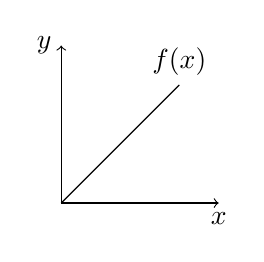
\begin{tikzpicture}
\draw[->] (0,0) -- (2,0) node [pos=1.0,below] {\(x\)};
\draw[->] (0,0) -- (0,2) node [pos=1.0,left] {\(y\)};
\draw (0,0) -- (1.5,1.5) node [pos=1.0,above] {\(f(x)\)};
\end{tikzpicture}
\caption{This is great caption}\label{figure}
\end{figure}\\
If you want to know more, check: \url{https://en.wikibooks.org/wiki/LaTeX/PGF/TikZ}.

%% If you want to include figure:
%\includegraphics[scale=1.0]{filename}
%% check https://en.wikibooks.org/wiki/LaTeX/Importing_Graphics if you want to know more

\end{document}
